% 15至45分钟一般报告.tex
% 根据 generic-ornate-15min-45min.en.tex,v 1.4 2004/10/07 20:53:08 tantau Exp 改编

\documentclass[cjk]{beamer}
\usepackage{pifont}
\usepackage{mathrsfs}
\usepackage{amsfonts}
\usepackage{xcolor}
\usepackage{harmony}
\usepackage{wasysym}
\usepackage{pifont}
\usepackage{graphicx}
\beamertemplateballitem
 \mode<presentation> {
  \usetheme{Warsaw}
  %\usetheme{Dresden}
  % 可以改成别的主题 Berkeley, PaloAlto, Goettingen, Marburg, Hannover,Berlin,
    %Ilmenau, Dresden, Darmstadt, Antibes, JuanLesPins, Montpellier
    %Frankfurt, Singapore, Szeged,Copenhagen, Luebeck, Malmoe,Warsaw Return to Theme


  \usecolortheme{default}
  \setbeamercovered{transparent}}
  %\setbeamercolor{frametitle}{fg=white,bg=blue!30}
   %标题元素颜色
  %\beamertemplateshadingbackground{blue!10}{yellow!5}
   %背景颜色渐变

%\transsplitverticalout
%\transdissolve<5>
%\transwipe
%\transsplithorizontalout

\setbeamertemplate{itemize items}{\color{blue!75!black}\blacksmiley}%\AAcht}%\ding{46}%\Vier}%\Acht}
%笑脸item
\usepackage{CJK}
% 如果内容中用到定理环境, 则需插入以下命令
\begin{CJK*}{GBK}{kai}
\newtheorem{thm}[theorem]{定理}
\newtheorem{lem}[theorem]{引理}
\end{CJK*}

\newcommand{\mbb}{\mathbb}
\newcommand{\Dlt}{\Delta}
\newcommand{\ptl}{\partial}
\newcommand{\al}{\alpha}
\newcommand{\be}{\beta}
\newcommand{\for}{\mbox{for}}
\newcommand{\vs}{\varsigma}
\newcommand{\stl}{\stackrel}
\newcommand{\vf}{\varphi}
\newcommand{\td}{\tilde}
\newcommand{\sgm}{\sigma}
\newcommand{\es}{\epsilon}
\newcommand{\la}{\langle}
\newcommand{\ra}{\rangle}
\newcommand{\dg}{\dag}
\newcommand{\nb}{\nabla}
\newcommand{\ka}{\kappa}
\newcommand{\raw}{\rightarrow}
\newcommand{\nn}{\nonumber}
\newcommand{\epa}{\varepsilon}
\newcommand{\gt}{\geqslant}
\newcommand{\lt}{\leqslant}
\newcommand{\sch}{Schr\"odinger }
\newtheorem{defnm}{定义}[section]
\newcommand{\Small}{\fontsize{10pt}{\baselineskip}\selectfont}
\newcommand{\smalll}{\fontsize{8.5pt}{\baselineskip}\selectfont}
\newcommand{\smallll}{\fontsize{8pt}{\baselineskip}\selectfont}

\begin{document}
\begin{CJK*}{GBK}{kai}
\CJKtilde




\title[{\bf 数据挖掘}]{\bf{\LARGE {\textcolor{blue!75!black}{数据挖掘十大算法之——K均值}}}}
% 如果标题不长, [短标题]可以略去

%\subtitle {{{\textcolor{blue!75!black\bf{\LARGE K\"ahler 流形上的KdV几何流}}}}}%{,red!75!black}

\author[{\bf 倪旭君}] % (如果作者不多, 则可略去此方括号)
{\bf {\large{倪旭君}} %\inst{1}
%\and 作者乙\inst{2}
}
% \inst{?} 仅用于有多个单位的情形

\institute[概率统计一年级] % (方括号内的简称是可以略去的)
{
\inst{1}
应用数学学院\\
  概率统计专业\\
硕士一年级
  %\and
  %\inst{2}%
  %某乙大学\\
  %计算机科学系
  }
% \inst 仅用于有多个单位的情形

\date[] % (方括号内的会议简称是可以略去的)
{ }

% 如果你想插入学校的徽章, 其文件名为 "university-logo-filename.xxx",
% 其中 xxx 是 pdflatex 能接受的格式, 则可用以下命令插入
% \pgfdeclareimage[height=0.5cm]{university-logo}{university-logo-filename}
% \logo{\pgfuseimage{university-logo}}

% 如果你想要在每一小节之前都显示一下目录, 则可把一下小段的注解号 "%" 删去
%\AtBeginSubsection[]
%{
%  \begin{frame}<beamer>
%    \frametitle{概要}
%    \tableofcontents[currentsection,currentsubsection]
%  \end{frame}
%}

% 除掉以下命令的注解 "%" 后, 许多环境都会自动逐段显示
%\beamerdefaultoverlayspecification{<+->}

\setbeamertemplate{title page}
{
\begin{center}
  %{\usebeamerfont{title}\usebeamercolor[fg]{title}\color{black}
  \textbf{\color{black}\inserttitle}
\vskip.8cm {\color{black}\insertauthor}\vskip.2cm {\small
 %\inst{1}%
中央财经大学\\
  %\vskip.3cm
  硕士一年级
  %\and
  %\inst{2}%
  %某乙大学\\
  %计算机科学系
  }
\insertdate
\end{center}
}




\begin{frame}
 \titlepage
 %\maketitle
\end{frame}

\begin{frame}
 \frametitle{数据挖掘十大算法之——K均值}
 \tableofcontents
  % 你也可以插入选项 [pausesections]
\end{frame}
  %以上这段用于生成目录页面

% 以下的演示文稿仅供参考, 不过可以提供一些忠告:
% - 除总结外, 最好不超过 3 节;
% - 每节至多分成 3 小节;
% - 每屏约 30 秒至 2 分钟, 因此总共 15 至 30 屏为佳.



\section{引入}

\begin{frame}{引言——聚类分析}
\

{\bf{\color{red!75!black}{\large Q:}}}\ 什么是聚类分析?

\

\ \ \ \ 聚类分析(Cluster Analysis)是根据\textcolor{red}{“物以类聚”}的道理,对样品或指标进行分类的一种多元统计分析方法,
它是\textcolor{blue}{在没有先验知识的情况下},对样本按各自的特性来进行合理的分类。

\end{frame}

\begin{frame}{系统地说}
  \ \ \ \ 聚类分析(cluster analysis)简称聚类~(clustering),是一个把数据对象\textcolor{blue}{划分}为子集的过程。每个子集是一个簇(cluster),使得簇中的对象彼此相似。
  \textcolor{blue}{划分}不是通过人来完成,而是依靠机器的计算,通过聚类算法实现。聚类对于处理大量不熟悉的数据是非常有用的,因为它能导致数据内
  实现未知的群组的发现。
\end{frame}


\begin{frame}{聚类分析的应用}

\ \ \ \ 聚类分析被应用于很多方面,在商业上,聚类分析被用来发现不同的客户群,并且通过购买模式刻画不同的客户群的特征;

\ \ \ \ 在生物上,聚类分析被用来动植物分类和对基因进行分类,获取对种群固有结构的认识;
在因特网应用上,聚类分析被用来在网上进行文档归类来修复信息。

\end{frame}

\begin{frame}{有、无监督学习——分类、聚类}
  \ \ \ \ 从机器学习的角度讲,簇相当于隐藏模式。聚类是搜索簇的无监督学习过程。与分类不同,无监督学习不依赖预先定义的类或带类标记的训练实例,
  需要由聚类学习算法自动确定标记,而分类学习的实例或数据对象有类别标记。聚类是观察式学习,而不是示例式的学习。
\end{frame}

\begin{frame}{聚类分析的分类}
\
{\bf{\color{red!75!black}{\large Q:}}}\ 聚类分析常见的有哪些方法?

\

\begin{itemize}
  \item 层次聚类。
  \item \textcolor{blue}{K均值聚类}。
  \item 密度聚类。
\end{itemize}

\end{frame}




\section{层次聚类}
\begin{frame}{层次聚类}
\ \ \ \ \textcolor{blue}{层次聚类}又称为系统聚类,首先要定义样本之间的\textcolor{red}{距离关系},距离较近的归为一类,较远的则属于不同的类。
可用于定义“距离”的统计量包括了欧氏距离(euclidean)、马氏距离(manhattan)、
两项距离(binary)、明氏距离(minkowski)。还包括相关系数和夹角余弦。
\end{frame}
\begin{frame}{层次聚类计算步骤}
\ \ \ \ 层次聚类\textcolor{red}{首先}将每个样本单独作为一类,\textcolor{blue}{然后}将不同类之间距离最近的进行合并,合并后重新计算类间距离。
这个过程一直持续到将所有样本归为一类为止。在计算类间距离时则有六种不同的方法,
分别是最短距离法、最长距离法、类平均法、重心法、中间距离法、离差平方和法。
\end{frame}

\begin{frame}{演示案例}
\ \ \ \ 下面我们用iris数据集来进行聚类分析,在R语言中所用到的函数为\textcolor{red}{hclust}。
首先提取iris数据中的4个数值变量,然后计算其欧氏距离矩阵。然后将矩阵绘制热图,从图中可以看到颜色越深表示样本间距离越近,
大致上可以区分出三到四个区块,其样本之间比较接近。
  %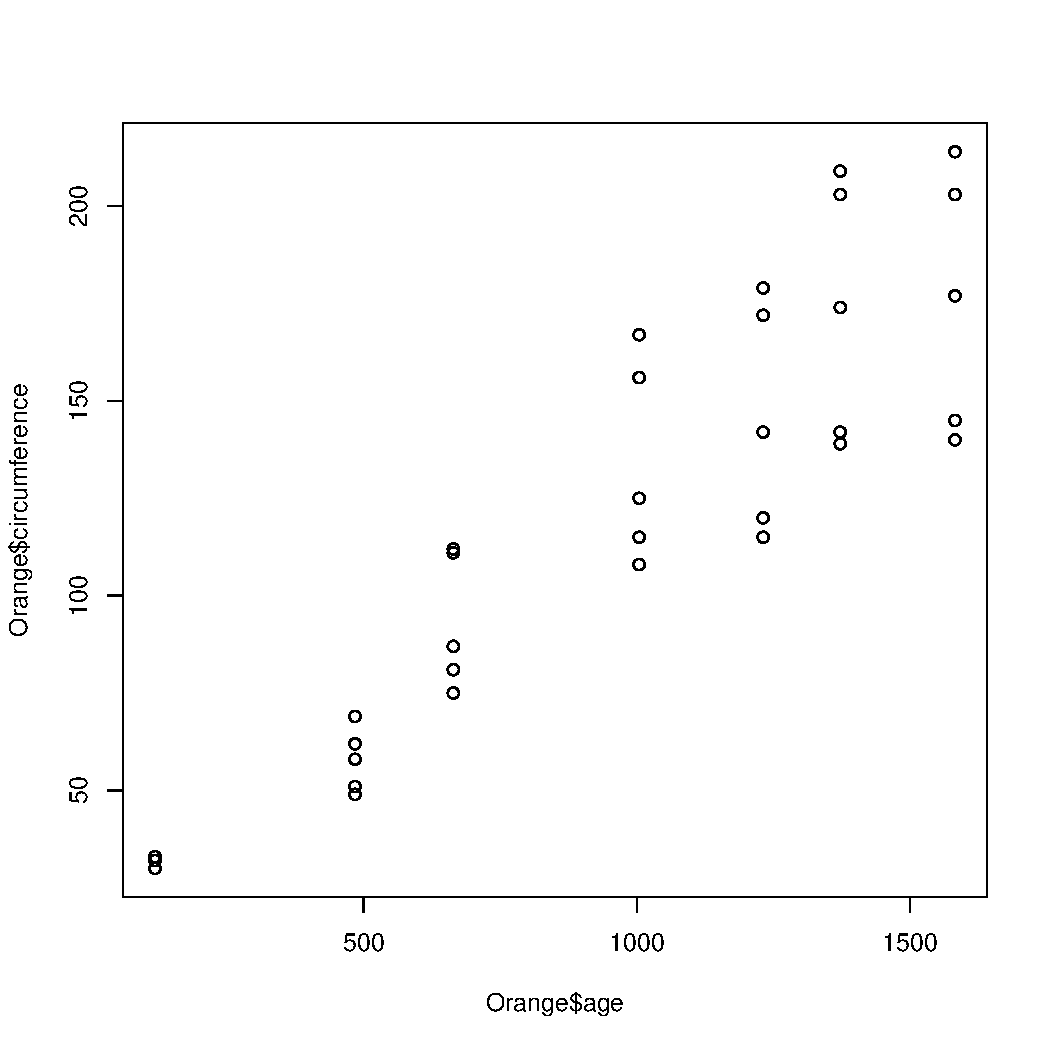
\includegraphics[scale=0.3]{1.png}\\

\end{frame}


\begin{frame}{效果如图}
\centering
\includegraphics[scale=0.4]{12.png}
\end{frame}

\section{K均值聚类}

\begin{frame}{K均值聚类}
\ \ \ \ K均值聚类又称为\textbf{动态聚类},它的计算方法较为简单,也不需要输入距离矩阵。
首先要指定聚类的分类个数N,随机取N个样本作为初始类的中心,计算各样本与类中心的距离并进行归类,
所有样本划分完成后重新计算类中心,重复这个过程直到类中心不再变化。

\ \ \ \ 顾名思义,K-means就是有K个中心,就是要把N个数据点分成K组。

\ \ \ \ 在R中使用kmeans函数进行K均值聚类,centers参数用来设置分类个数,nstart参数用来设置取随机初始中心的次数,
其默认值为1,但取较多的次数可以改善聚类效果。model2\$cluster可以用来提取每个样本所属的类别。
\end{frame}



\begin{frame}{如下图所示:}
\begin{center}
 \includegraphics[scale=0.28]{2.png}
\end{center}
 \ \ \ \   很明显看得出来这些点分成三类。但是人能看出来,不代表计算机也看得出来。机器学习的目的就是在于,让计算机不仅可以实现1+1=2这样的计算问题,
 也能做一些模式识别、数据挖掘这样的需要一点智能的工作。
\end{frame}

\begin{frame}{K均值的做法-1}
\begin{center}
\includegraphics[scale=0.3]{3.png}
\end{center}
\ \ \ \ 为了找出这三类点,首先我要在这个区域中间任取三个点作为三个类的中心。比如,我在所有的数据点中间任选三个:
\end{frame}

\begin{frame}{K均值的做法-2}
  当然,这三个点肯定不是我最后要找到的中心。所以要采用迭代的方法:

  \begin{eqnarray}
    S_i^{(t)}=\{x_j: \|x_j -m_i^{(t)}\| \leq \|x_j -m_{i^*}^{(t)}\| for \  all \  i^*=1,...,k \}  \\
    m_i^{(t+1)}=\frac{1}{S_i^{(t)} \sum_{X_j \in S_i^{(t)}} X_j}
  \end{eqnarray}

  这个是wikipedia上面对K-means核心算法的解释。就是根据第t次得到的中心,把所有数据点进行分类。
  然后每一类的新的中心就是这类点的重心。显然,这个算法最后一定会收敛。
\end{frame}


\begin{frame}{K均值的做法-3}
\begin{center}
  \includegraphics[scale=0.3]{4.png}
  \end{center}
  这个是一次迭代的效果,箭头的方向是迭代路径。
\end{frame}

\begin{frame}{K均值的做法-4}
  最后的分类:
\begin{center}
  \includegraphics[scale=0.3]{5.png}
  \end{center}
  但是,k-means并不是一个好的算法。原因是它太依赖于对初始值的选择了。而且比较慢。
\end{frame}

\begin{frame}{K均值的缺点-错误分类}
  比如下图就是一次错误的分类,红色和蓝色的初值取的太近。所以把左下角的一大片点都看作是绿色的了。
\begin{center}
  \includegraphics[scale=0.3]{6.png}
\end{center}
\end{frame}

\begin{frame}{K均值的缺点-错误分类}
  \ \ \ \ 六组的时候就更悲剧了……
\begin{center}
  \includegraphics[scale=0.33]{7.png}
\end{center}
\end{frame}
\begin{frame}
\ \ \ \ 随着组类别的增加,K均值算法的\textcolor{blue}{计算量}(复杂度)会显著上升,这不仅仅体现在算法复杂度上(K均值算法的复杂度为\textcolor{red}{O(nkt)}),而是在于
初始样本中心给定方式过于杂乱无章, 造成计算量增大。
\end{frame}

\begin{frame}{K均值的做法-总结}
  \ \ \ \ K均值聚类(K-means clustering)计算简单,并且可以用于各种数据类型,但需要事先判断簇个数来作为输入参量,
  该参数的设置往往涉及到聚类效果。

  \ \ \ \ 现实生活中,需要处理的维数往往非常大。很多时候,\textcolor{blue}{这个算法只能得到局部最优解},
  要\textcolor{red}{重复试验很多次}才可以得到真实的聚类。所以,只有对初始值的选取规则进行一定的优化才可以提高这个算法的效率。
\end{frame}



%\begin{frame}{结果展示}
%\begin{center}
%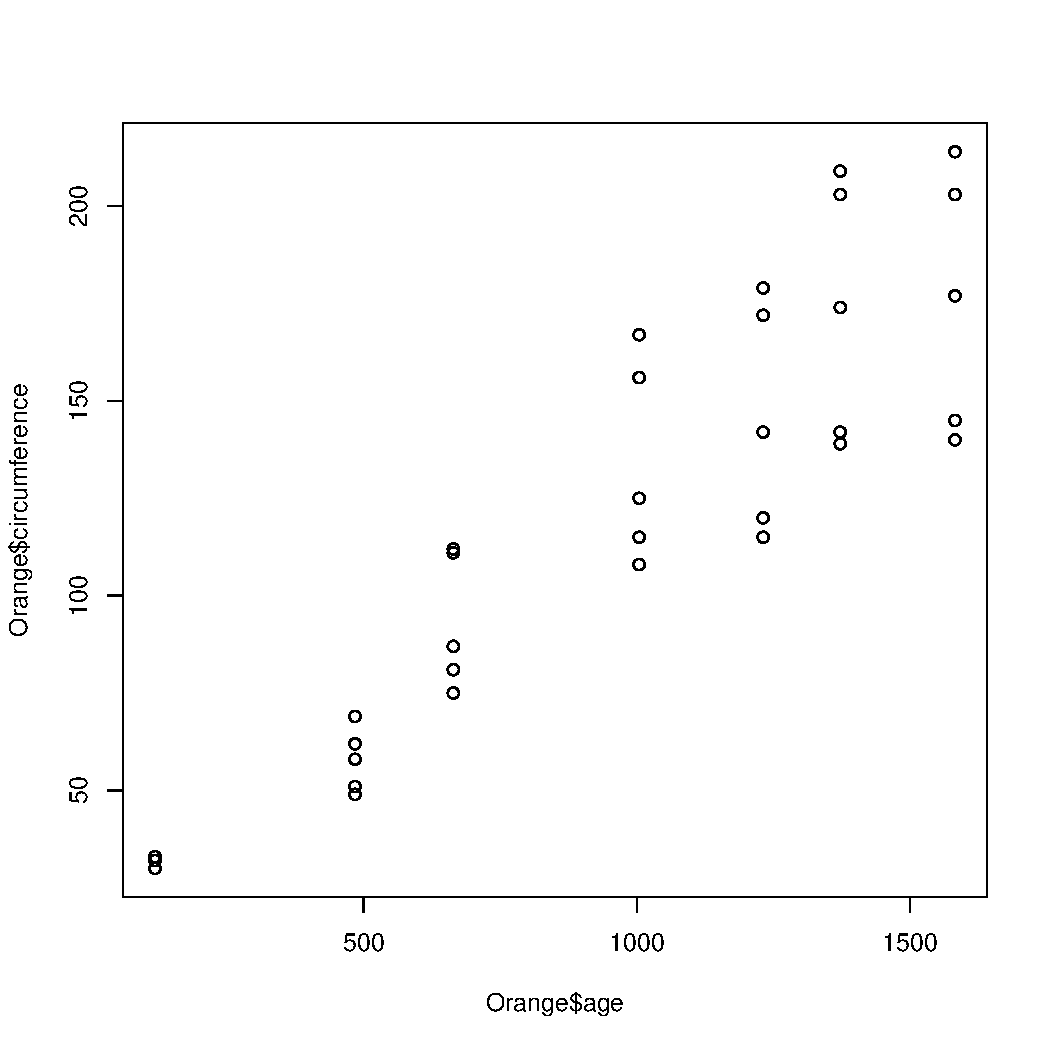
\includegraphics[scale=0.4]{1.png}
%\end{center}
%\end{frame}


\begin{frame}{几点需要注意的}
\ \ \ \ 使用K均值聚类时需要注意,只有在类的平均值被定义的情况下才能使用,还要求事先给出分类个数。
一种方法是先用层次聚类以决定个数,再用K均值聚类加以改进。或者以轮廓系数来判断分类个数。
改善聚类的方法还包括对原始数据进行变换,如对数据进行降维后再实施聚类。

\ \ \ \ cluster扩展包中也有许多函数可用于聚类分析,如agnes函数可用于凝聚层次聚类,
diana可用于划分层次聚类,pam可用于K均值聚类,fanny用于模糊聚类。
\end{frame}

\section{扩展}

\begin{frame}{轮廓系数}
\ \ \ \ K均值聚类(K-means clustering)计算简单,并且可以用于各种数据类型,但需要事先判断簇个数来作为输入参量,
该参数的设置往往涉及到聚类效果。

\ \ \ \ 轮廓系数可以用来解决这个问题,轮廓系数(silhouette coefficient)方法结合了凝聚度和分离度,可以以此来判断聚类的优良性,其值在-1到+1之间取值,值越大表示聚类效果越好。

\ \ \ \ 依据这个原理,我们可以尝试用多个簇参量,反复计算在每个簇个数条件下的轮廓系数,
当轮廓系数取最大时,其相应的簇个数是最好的。


\end{frame}


\begin{frame}{轮廓系数的R语言实现}
\ \ \ \ 在R语言中package fpc可以计算聚类后的一些评价指标,其中就包括了轮廓系数。
\end{frame}

\begin{frame}{K均值算法的另一个不足}
  \ \ \ \

  \ \ \ \ K均值聚类使用非常广泛,作为最为古老的聚类方法,它的算法非常简单,而且速度很快。
  但是其缺点在于它不能识别非球形的簇。我们可以用一个简单的例子来观察K均值聚类的弱点。
\end{frame}

\begin{frame}{例子}
\ \ \ \ 我们先构造一些人为数据,它是基于sin函数和cos函数构成的两组点。
如果我们用传统的K均值聚类,结果如下图所示。其聚类结果是不理想的,因为它不能识别非球形的簇。
\begin{center}
\includegraphics[scale=0.3]{9.png}
\end{center}
\end{frame}

\begin{frame}{解决办法——DESCAN(密度聚类)算法}
  \ \ \ \ 为了解决这个问题,我们可以使用DBSCAN方法,它是一种基于密度的聚类方法。即寻找那些被低密度区域所分离的高密度区域。

\ \ \ \
DBSCAN方法的重要概念如下:

\begin{itemize}
  \item 核心点:如果某个点的邻域内的点的个数超过某个阀值,则它是一个核心点,
      即表示它位于簇的内部。邻域的大小由半径参数eps决定。阀值由MiniPts参数决定。
  \item 边界点:如果某个点不是核心点,但它落在核心点的邻域内,则它是边界点。
  \item 噪声点:即非核心点也非边界点。
\end{itemize}

\end{frame}


\begin{frame}{图示}
\begin{center}
  \includegraphics[scale=0.4]{10.jpg}
  \end{center}
  在上图中,红色的点均为核心点,黄色的为边界点,而蓝色的则为噪声点。
\end{frame}

\begin{frame}{简单的说}
  \ \ \ \ 简单来讲,\textcolor{red}{DBSCAN}的算法是\textcolor{blue}{将所有点标记为核心点、边界点或噪声点,将任意两个距离小于eps的核心点
  归为同一个簇。任何与核心点足够近的边界点也放到与之相同的簇中}。应用R语言中的fpc包来对上面的例子实施密度聚类。
  其中eps参数设为0.6,即两个点之间距离小于0.6则归为一个簇,而阀值MinPts设为4。
\end{frame}

\begin{frame}{效果图}
\begin{center}
\includegraphics[scale=0.2]{11.png}
\end{center}
从上图可以看到,DBSCAN方法很好的划分了两个簇。其中要注意参数eps的设置,如果eps设置过大,则所有的点都会归为一个簇,
如果设置过小,那么簇的数目会过多。如果MinPts设置过大的话,很多点将被视为噪声点。

\end{frame}

\begin{frame}{总结}
  \begin{itemize}
    \item K均值作为一种原理清晰简单的无监督学习方法,在计算应用中非常广泛,但是聚类效果依靠于对类数的设定和初始点的产生,当初始点产生
        位置不理想时,K均值的计算量会变大,特别是在多分类计算时,算法的劣势就显现了。
    \item  虽然类数可以通过轮廓系数的方法来解决,但是K均值在区分不规则群落数据时(参考最后一个例子),效果不好。 从最后一个例子中,我们可以发现K均值聚类算法的缺点,而基于密度聚类的具有相对优良特性,它可以对抗噪声,能处理任意形状和大小的簇。
        但是对于高维数据,点之间极为稀疏,密度就很难定义了。
    \item 在K-Means算法中,使用的距离概念是欧式距离,这个\textcolor{red}{必须在欧式空间中才有效}。
        这个对数据的要求比较高,
        如果不能使用欧式空间内的距离(Distance)来描述数据点之间的差异(Dissimilarity),K-Means算法就无能为力。
  \end{itemize}
\end{frame}

\begin{frame}{总结}
    \begin{itemize}
      \item 聚类分析是一种\textcolor{red}{无监督学习方法},目的是捕获数据的自然结构,从而将数据划分为有意义的组。
        聚类分析还可以用来对大数据进行预处理,为进一步的数据挖掘工作起到\textcolor{blue}{压缩}和\textcolor{blue}{降维}
        的作用。
    \end{itemize}
\end{frame}

\section*{Thanks}
\begin{frame}

\begin{center}
%  \includegraphics[height=3.5in,width=5in]{thanksblue.jpg}%\pause
%\end{center}
%\begin{center}
 % \only<2->{\includegraphics[width=2.0in]{curve2.jpg}}
\end{center}
\vspace{1cm} {\centerline{\Huge Thanks!}}
\end{frame}



\end{CJK*}
\end{document}
